\documentclass[11pt]{article}
\usepackage{graphicx}
\usepackage{geometry}

\geometry{
	left=25mm,
	right=25mm,
	top=25mm,
	bottom=25mm,
}
\begin{document}
	
	\begin{center}
		\textbf{ASSIGNMENT– 6}
	\end{center}
	\textbf{AIM:}
	Implement Apriori approach for data mining to organize the data items on a shelf using
	following table of items purchased in a Mall \\ 
	
	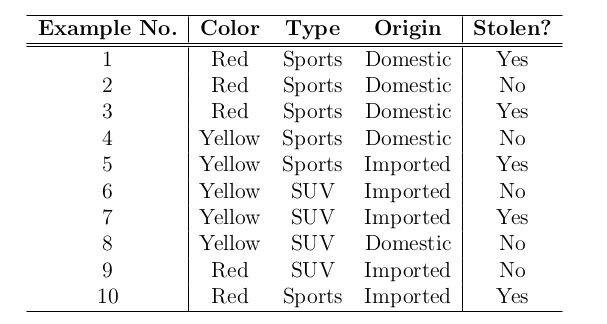
\includegraphics{image1}
	
	
	\noindent \textbf{OBJECTIVE:}
	\begin{itemize}
		\item To understand the basic concept of Apriori algorithm.
		\item To implement Apriori Algorithm.
	\end{itemize}
	
	\noindent \textbf{SOFTWARE REQUIREMENTS:}
	\begin{itemize}
		\item Linux Operating System
		\item Weka Tool
	\end{itemize}•
	
	\noindent \textbf{MATHEMATICAL MODEL:} \\
	Consider a set S consisting of all the elements related to a program. \\
	The Mathematical model is given as below, \\
	S={s,e,X,Y,Fme,DD,NDD,Mem shared } \\
	Where, \\
	s = Initial State \\
	e = End State \\
	X = Input. Here it is number of elements, actual element \\
	Y = Output. Here output is frequent patterns \\
	Fme = Algorithm/Function used in program. for eg. fcal mean(),cal di()g \\
	DD=Deterministic Data \\
	NDD=Non deterministic Data \\
	Mem shared=Memory shared by processor. \\
	
	\noindent \textbf{THEORY:} \\
	\paragraph{}
	Apriori is an algorithm for frequent item set mining and association rule learning over
	transactional databases. It proceeds by identifying the frequent individual items in the database
	and extending them to larger and larger item sets as long as those item sets appear sufficiently
	often in the database. The frequent item sets determined by Apriori can be used to
	determine association rules which highlight general trends in the database: this has applications
	in domains such as market basket analysis.
	\paragraph{}
	The Apriori algorithm was proposed by Agarwal and Srikant in 1994. Apriori is designed to
	operate on databases containing transactions (for example, collections of items bought by
	customers, or details of a website frequentation). Other algorithms are designed for finding
	association rules in data having no transactions, or having no timestamps (DNA sequencing).
	Each transaction is seen as a set of items (an item set). Given a threshold, the Apriori algorithm
	identifies the item sets which are subsets of at least transactions in the database.
	\paragraph{}
	Apriori uses a "bottom up" approach, where frequent subsets are extended one item at a time (a
	step known as candidate generation), and groups of candidates are tested against the data. The
	algorithm terminates when no further successful extensions are found.
	\paragraph{}
	Apriori uses breadth-first search and a Hash tree structure to count candidate item sets
	efficiently. It generates candidate item sets of length from item sets of length . Then it prunes the
	candidates which have an infrequent sub pattern. According to the downward closure lemma, the
	candidate set contains all frequent -length item sets. After that, it scans the transaction database
	to determine frequent item sets among the candidates.
	
	\begin{itemize}
		\item The pseudo code for the algorithm is given below for a transaction database, and a
		support threshold of. Usual set theoretic notation is employed; though note that is a musti
		set. is the candidate set for level . At each step, the algorithm is assumed to generate the
		candidate sets from the large item sets of the preceding level, heeding the downward
		closure lemma. Accesses a field of the data structure that represents candidate set , which
		is initially assumed to be zero. Many details are omitted below, usually the most
		important part of the implementation is the data structure used for storing the candidate
		sets, and counting their frequencies.
	\end{itemize}
	
	\begin{center}
		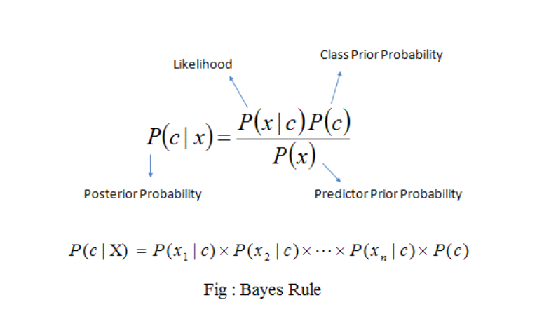
\includegraphics{204/assign6(apriori)/image1.png} \\
		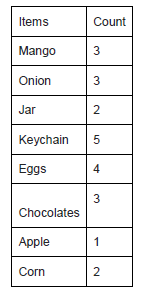
\includegraphics{204/assign6(apriori)/iamge2.png} \\
		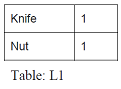
\includegraphics{204/assign6(apriori)/iamge3.png} \\
		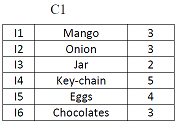
\includegraphics{204/assign6(apriori)/iamge4.png} \\
		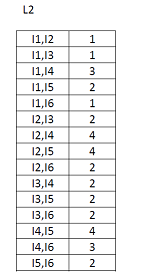
\includegraphics{204/assign6(apriori)/iamge5.png} \\
		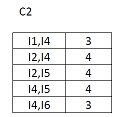
\includegraphics{204/assign6(apriori)/iamge6.png} \\
		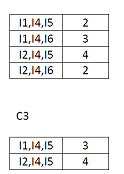
\includegraphics{204/assign6(apriori)/iamge7.png} \\
	\end{center}
	
	Hence these are the item sets which occurred frequently in the database . \\
	
	\noindent \textbf{ CONCLUSION:}
	Thus, we have implemented Apriori Algorithm.
	
	\begin{center}
		\begin{tabular}
			{|c|c|c|c|c|}\hline
			{\bf Roll No.}		&{\bf Name of Student}	&{\bf Date of Performance}  				&{\bf Date of Submission}	&{\bf Sign.}  \\    \hline
			BECOC357	& Sunny Shah  & 21 / 09 / 2017		& 28 / 09 / 2017		&  \\ \hline
		\end{tabular}\\ 
	\end{center}
	
\end{document}
